\documentclass[preprint]{article}


\PassOptionsToPackage{numbers, compress}{natbib}


% ready for submission
\usepackage{neurips_2023}

\usepackage{microtype}
\usepackage{xcolor}
\usepackage{hyperref}
\usepackage{url}
%\usepackage{listings}
%\usepackage{pifont}
%\usepackage{tikz}
\usepackage{subfig}
\usepackage{multirow}
%\usepackage{pgfplots}
\usepackage{booktabs}
%\usepackage{dcolumn}
%\usepackage{cancel}
%\usepackage{ifmtarg}
%\usepackage{verbatim}
\usepackage{graphicx}
%\usepackage{chngpage}
\usepackage{xspace}
\usepackage{algorithm}
\usepackage[noend]{algpseudocode}
\usepackage{balance}
\usepackage{amsmath}
\usepackage{amssymb}
\usepackage{amsthm}
%\usepackage{times}
%\usepackage{fullpage}
%\usepackage{footnote}
%\usepackage[symbol]{footmisc}
\usepackage{threeparttable}
%\usepackage[small,compact]{titlesec}
%\usepackage{tabularx}
%\usepackage{titling}
%\usepackage{authblk}
%\makesavenoteenv{tabular}
%\makesavenoteenv{table}
\usepackage{cleveref}
\usepackage{mathtools}


\newcommand{\Sys}{SpecInfer\xspace}
\newcommand{\sys}{SpecInfer\xspace}
\newcommand{\llama}{LLaMA\xspace}
\newcommand{\m}{\mathcal}
\newcommand{\Continue}{\State {\bf continue}}
\newcommand{\ZJ}[1]{\textcolor{red}{ZJ: #1}}
\newcommand{\XM}[1]{\textcolor{blue}{XM: #1}}
\algnewcommand{\LineComment}[1]{\State \textcolor{violet}{\(\triangleright\) #1}}
\newcommand\blfootnote[1]{%
  \begingroup
  \renewcommand\thefootnote{}\footnote{#1}%
  \addtocounter{footnote}{-1}%
  \endgroup
}

%%%%%%%%%%%%%%%%%%%%%%%%%%%%%%%%
% THEOREMS
%%%%%%%%%%%%%%%%%%%%%%%%%%%%%%%%
\theoremstyle{plain}
\newtheorem{theorem}{Theorem}[section]
\newtheorem{proposition}[theorem]{Proposition}
\newtheorem{lemma}[theorem]{Lemma}
\newtheorem{corollary}[theorem]{Corollary}
\theoremstyle{definition}
\newtheorem{definition}[theorem]{Definition}
\newtheorem{assumption}[theorem]{Assumption}
\theoremstyle{remark}
\newtheorem{remark}[theorem]{Remark}


\title{Collie: Accelerating Generative LLM Serving\\with Tree-based Speculative Inference and Verification}

\begin{document}

%\date{}
%\maketitle

\begin{figure}
    \centering
    \subfloat[Greedy sampling.]{
    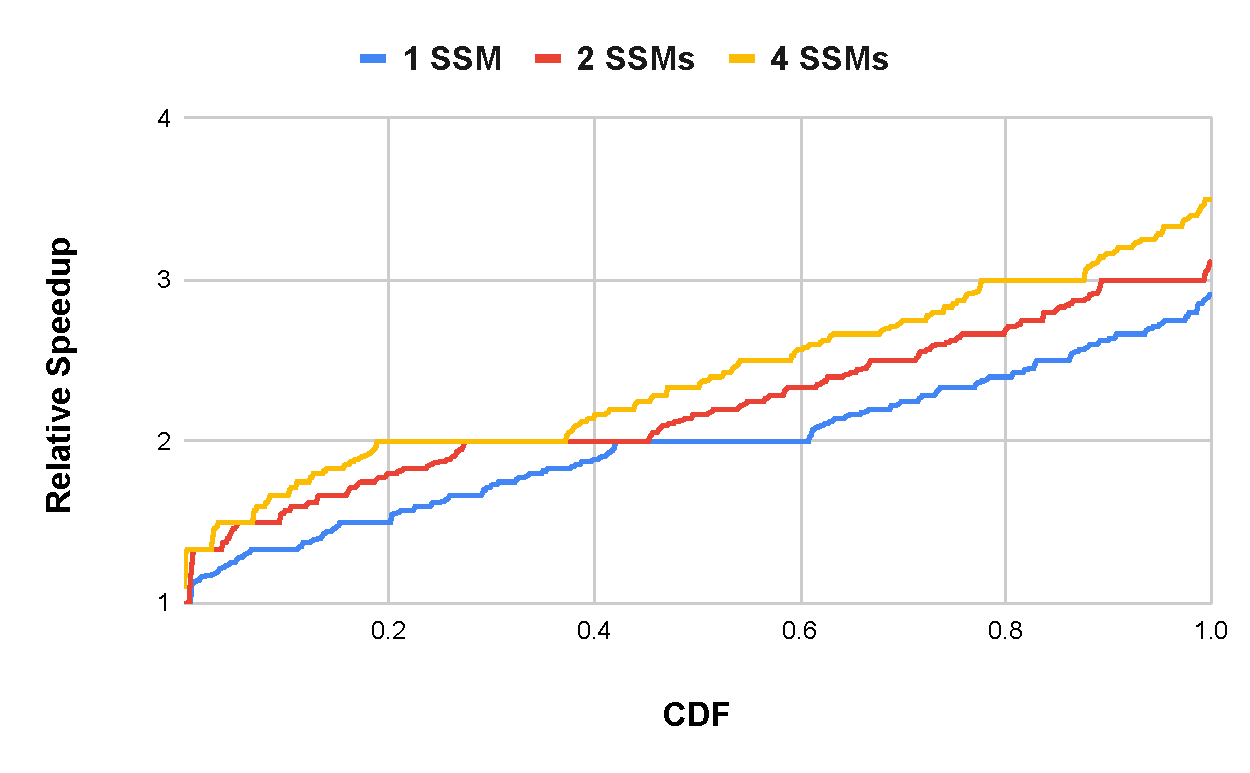
\includegraphics[scale=0.5]{rebuttal_figs/ssms_greedy_decoding.pdf}
    }
    \\
    \subfloat[Stochastic sampling.]{
    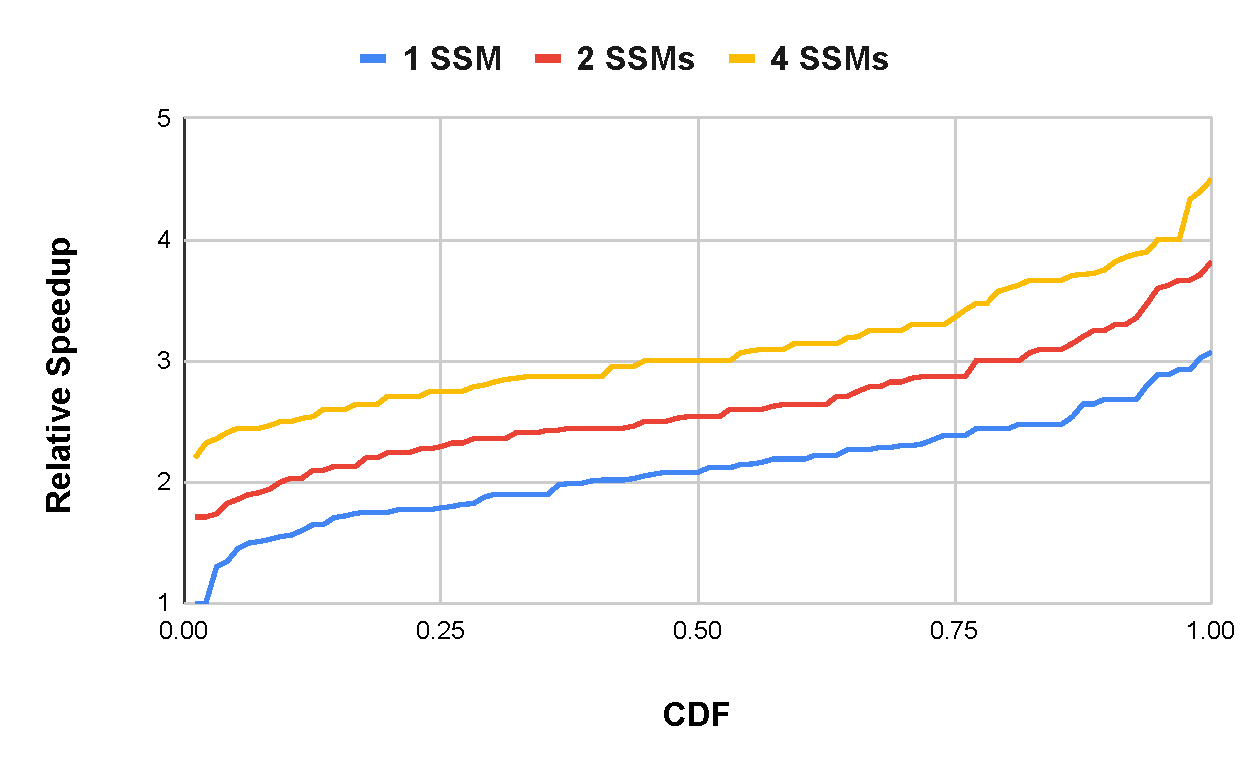
\includegraphics[scale=0.5]{rebuttal_figs/ssms_stochastic_decoding.pdf}
    }
    \caption{Comparing LLM inference performance of Collie with different numbers of SSMs. In this experiment, we serve the LLAMA-7B model on a single NVIDIA A10 GPU using a batch size of 1. 
    The figure shows the cumulative distribution function (CDF) of the relative speedup against incremental decoding (i.e., with on SSM) for prompts from the Alpaca dataset[33]. The blue curve shows the performance of existing speculative decoding baselines with a pre-trained LLAMA-160M model and sequence-based decoding. The red and yellow curves show Collie's performance using multiple collectively boost-tuned SSMs and tree-based parallel decoding.}
    \label{fig:ssms_greedy_coding}
\end{figure}

\begin{figure}
    \centering
    \subfloat[Latency (lower is better).] {
    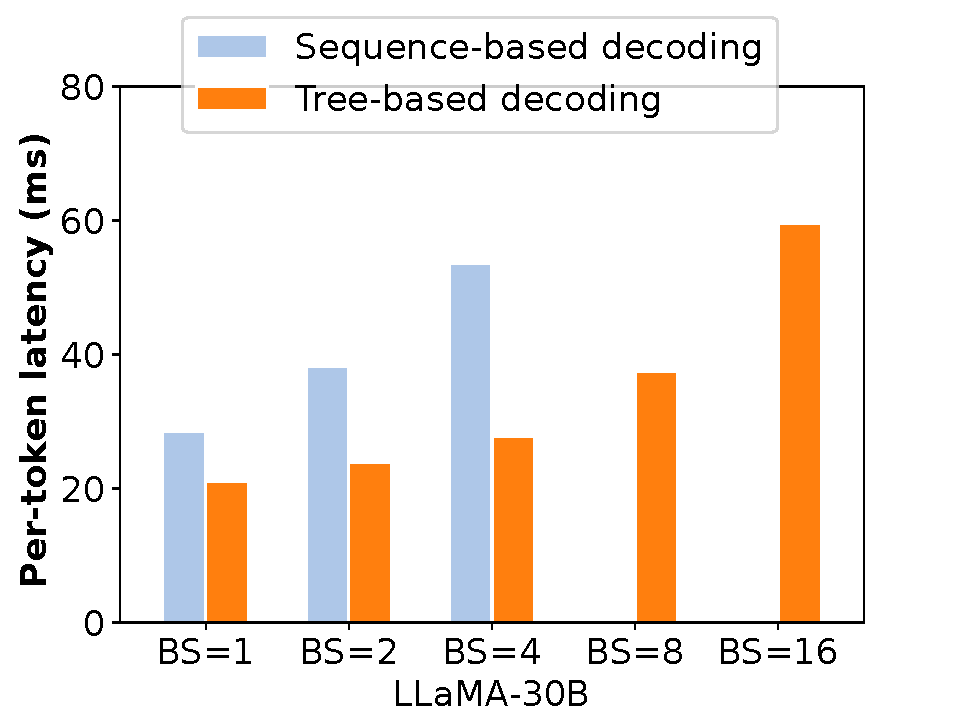
\includegraphics[scale=0.4]{rebuttal_figs/rebuttal_sequence_vs_tree_latency.pdf}
    }
    \subfloat[Throughput (higher is better).]{
    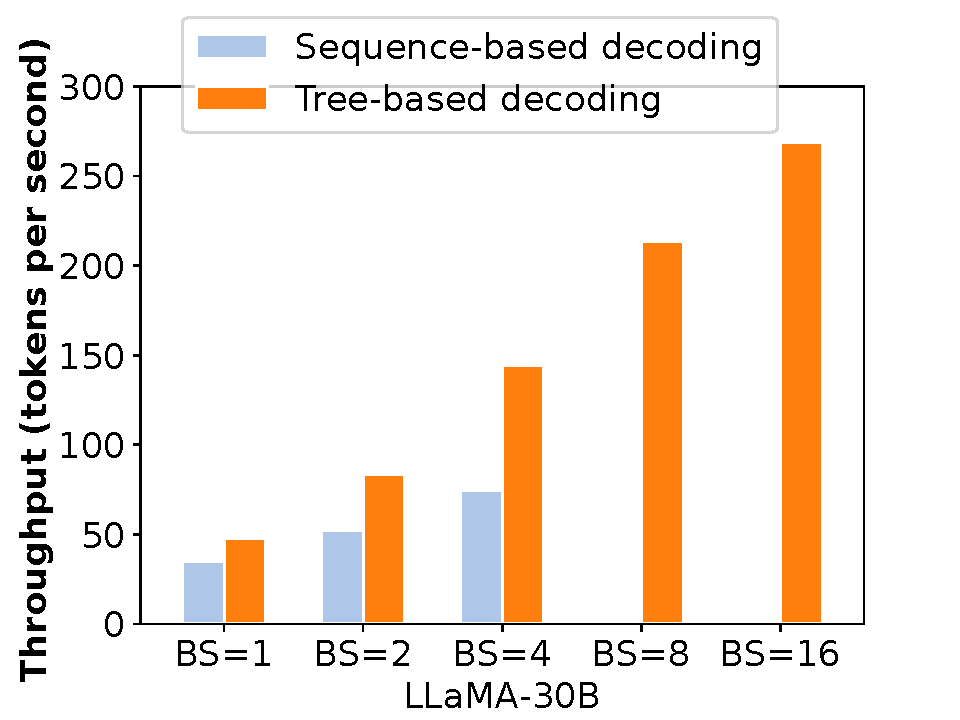
\includegraphics[scale=0.4]{rebuttal_figs/rebuttal_sequence_vs_tree_throughput.pdf}
    }
    \caption{Comparing the end-to-end inference latency and serving throughput of sequence-based and tree-based decoding on the Alpaca dataset[33]. We use LLAMA-30B as the LLM and 4 SSMs collectively boost-tuned from LLAMA-160M. We ran experiments on four NVIDIA A10 GPUs. Each GPU serves an SSM using data parallelism and the four GPUs jointly serve the LLM using tensor model parallelism. The sequence-based decoding approach cannot serve 8 requests in parallel due to the memory overhead of computing all 32 sequences (i.e., 4 sequences per request) during verification.}
    \label{fig:ssms_greedy_coding}
\end{figure}

\begin{figure}
    \centering
    \subfloat[Greedy sampling CDF.]{
    \includegraphics[width=0.33\linewidth]{figs/Greedy sampling CDF.pdf}
    }
    \subfloat[Stochastic sampling CDF.]{
    \includegraphics[width=0.33\linewidth]{figs/Stochastic sampling CDF.pdf}
    }
    \subfloat[Greedy decoding CDF.]{
    \includegraphics[width=0.33\linewidth]{figs/Greedy decoding CDF.pdf}
    }
    \caption{CDF figures of greedy sampling, stochastic sampling and greedy decoding.}
    \label{fig:ssms_greedy_coding}
\end{figure}

%\bibliographystyle{plain}
%\bibliography{reference}

\end{document}